\documentclass[11pt, oneside]{article}   	% use "amsart" instead of "article" for AMSLaTeX format
\usepackage[top=1.3in,bottom=1in,right=1in,left=1in,headheight=30pt]{geometry}

\geometry{letterpaper}                   		% ... or a4paper or a5paper or ...
%\geometry{landscape}                		% Activate for rotated page geometry
%\usepackage[parfill]{parskip}    		% Activate to begin paragraphs with an empty line rather than an indent
\usepackage{graphicx}				% Use pdf, png, jpg, or eps§ with pdflatex; use eps in DVI mode
\usepackage{pdfpages}
\usepackage{pgfplots, xcolor}
\usepackage{amsmath,amsthm,amssymb,amsfonts} 	%Prooflandia
\usepackage[utf8]{inputenc}
\usepackage{amssymb}
\makeatother
\usepackage{pifont}
\usepackage{marvosym, wasysym, graphicx, wrapfig, placeins, subcaption, booktabs}
 \usepackage{cancel, framed, topcapt}
 \usepackage{tikz, pgfplots, pifont}
 \usepackage [autostyle, english = american]{csquotes}
	\MakeOuterQuote{"}
\usepackage{fancyhdr}
\pagestyle{fancy}
\lhead{Modeling Complex Systems --- CSYS/CS 302\\
Assignment 01  \\
Date: \today
} %%%%%%%%%%%% PUT IN ASSIGNMENT # %%%%%%%%%%%%
\rhead{Sarah Howerter\\
Daniel Berenberg}
\cfoot{\thepage}

\usepackage[colorlinks=true, pdfstartview=FitV, linkcolor=blue,
            citecolor=blue, urlcolor=blue]{hyperref}
            \usepackage{color}
            \definecolor{dkgreen}{rgb}{0,0.6,0}
            \definecolor{gray}{rgb}{0.5,0.5,0.5}
            \definecolor{mauve}{rgb}{0.58,0,0.82}
            \usepackage{listings}
            \lstset{frame=tb,
              language=python,
              aboveskip=3mm,
              belowskip=3mm,
              showstringspaces=false,
              columns=flexible,
              basicstyle={\footnotesize\ttfamily},
              numbers=none,
              numberstyle=\tiny\color{gray},
              keywordstyle=\color{blue},
              commentstyle=\color{dkgreen},
              stringstyle=\color{mauve},
              breaklines=true,
              breakatwhitespace=true,
              tabsize=3
            }

\newcommand{\N}{\mathbb{N}}
\newcommand{\Z}{\mathbb{Z}}
\newcommand{\bt}{$\bullet$}
\newcommand{\cmdin}{$>$}
\newcommand{\cmdout}{[1]}
%SetFonts
%\, = insert small space
%\textrm{} = sets to text form inside math land
%SetFonts

\newcommand{\prob}[2]{
\indent \\
\noindent{\color{green!50!blue}\bf {\large#1.}}
{\normalfont #2}
}
\newcommand{\Prob}{\textrm{{\bf Pr}}}

\begin{document}
\prob{1}{See code. Filename: \texttt{numerical.py} \\
	\indent - line number: 38 for Euler's method \\
	\indent -  line number: 56 for Heun's method}

\prob{2}{Figure \ref{9_Lotka-Volterra_plots} shows the 3-species approximation for each of our parameter combinations of $\alpha$ and $h$. We observe that as our timestep spacing parameter $h$ increases, the Euler approximation gets worse. It only appears to be a sufficient method for estimating for the most stable case and highest resolution, $\alpha=0.75,h=0.1$. Particularly for the more chaotic parameter of $\alpha=1.5$ and the lowest resolution step size of $h = 1.0$, the Euler method completely diverges for all $x_i$ species, and even Heun's method is also a poor appriximation of the system behavior. }
	\hspace{-2mm}\begin{figure}[h!]
		\centering
		\begin{tabular}{lll}
			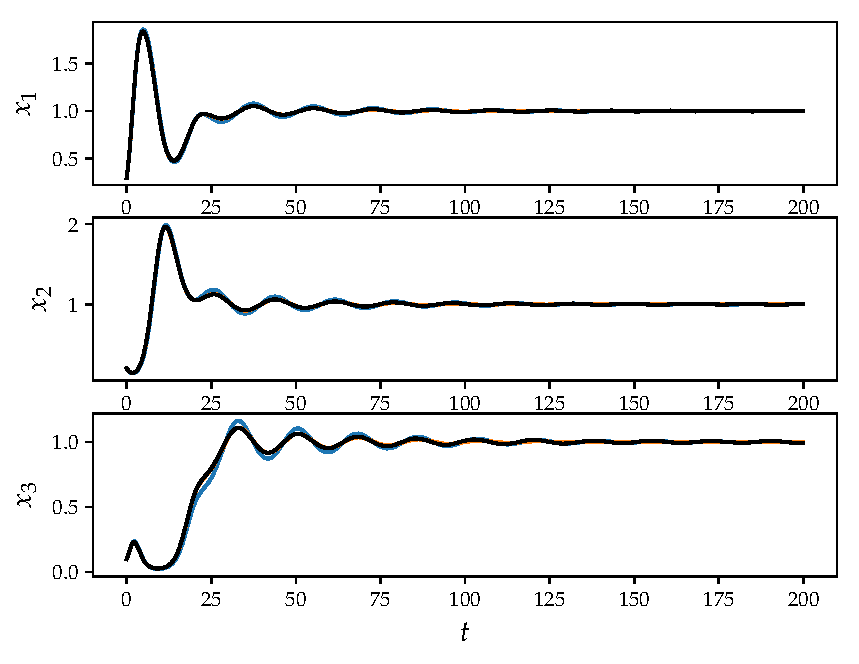
\includegraphics[width=0.35\textwidth]{figs/3SpeciesApprox75_1.pdf}
			&
			\hspace{-5mm}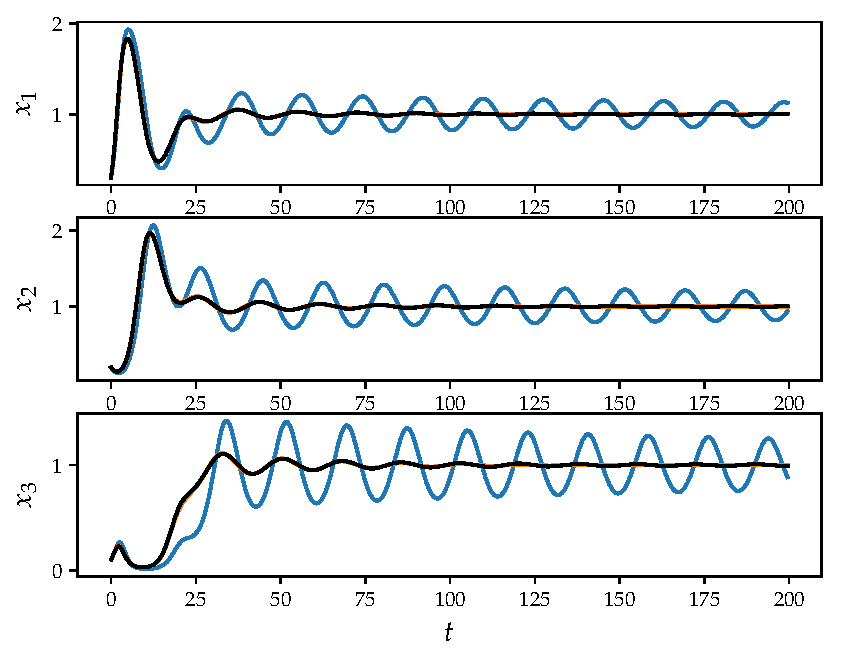
\includegraphics[width=0.35\textwidth]{figs/3SpeciesApprox75_5.pdf}
			&
			\hspace{-5mm}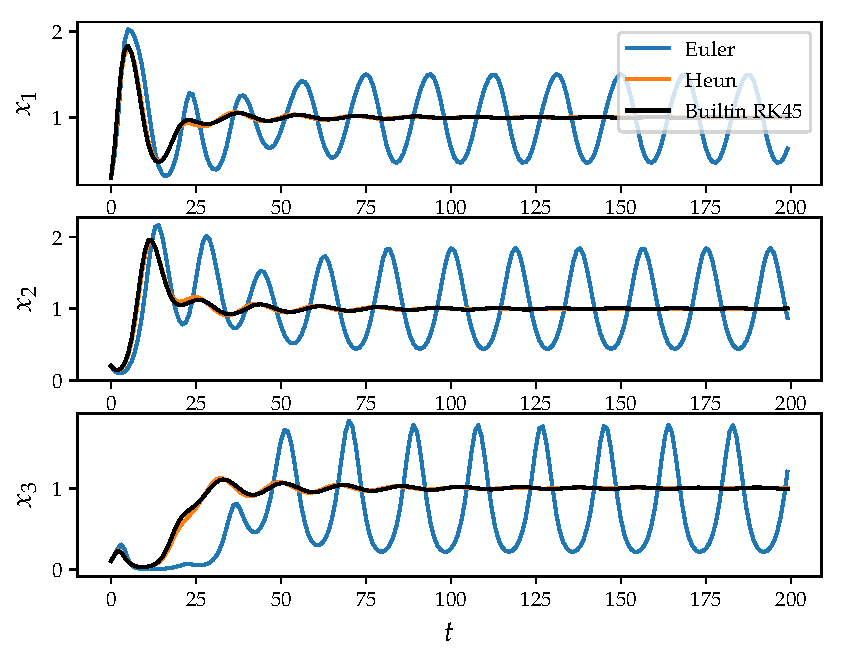
\includegraphics[width=0.35\textwidth]{figs/3SpeciesApprox75_10.pdf}\vspace{-3mm}
			\\
			{\scriptsize \hspace{4mm}(a) $\alpha = 0.75, h=0.1$} &
			{\scriptsize \hspace{4mm}(b) $\alpha = 0.75, h=0.5$}&
			{\scriptsize \hspace{4mm}(c) $\alpha = 0.75, h=1.0$}
			\\
			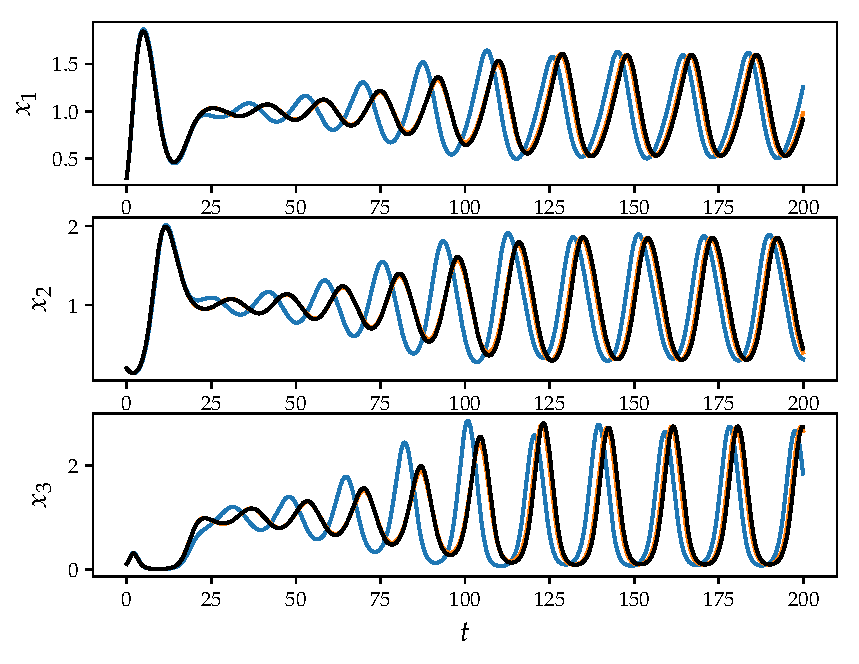
\includegraphics[width=0.35\textwidth]{figs/3SpeciesApprox120_1.pdf}
			&
			\hspace{-5mm}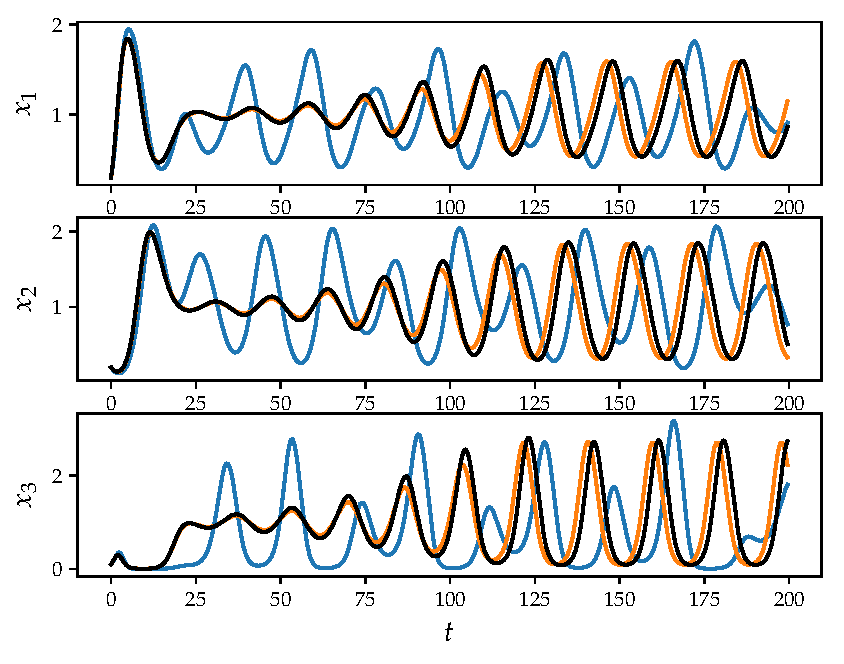
\includegraphics[width=0.35\textwidth]{figs/3SpeciesApprox120_5.pdf}
			&
			\hspace{-5mm}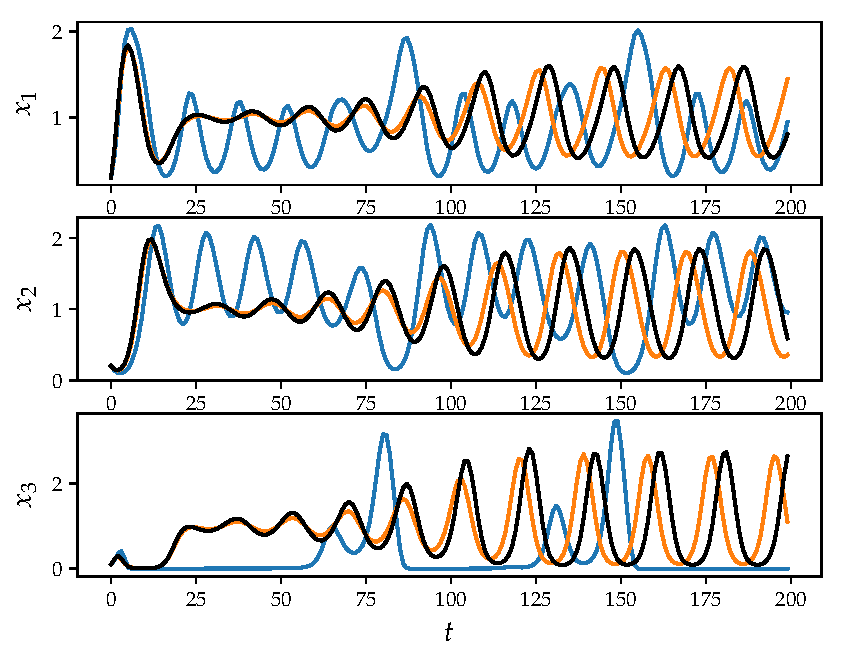
\includegraphics[width=0.35\textwidth]{figs/3SpeciesApprox120_10.pdf}\vspace{-3mm}
			\\
			{\scriptsize \hspace{4mm}(d) $\alpha = 1.20, h=0.1$}&
			{\scriptsize \hspace{4mm}(e) $\alpha = 1.20, h=0.5$}&
			{\scriptsize \hspace{4mm}(f) $\alpha = 1.20, h=1.0$}
			\\
			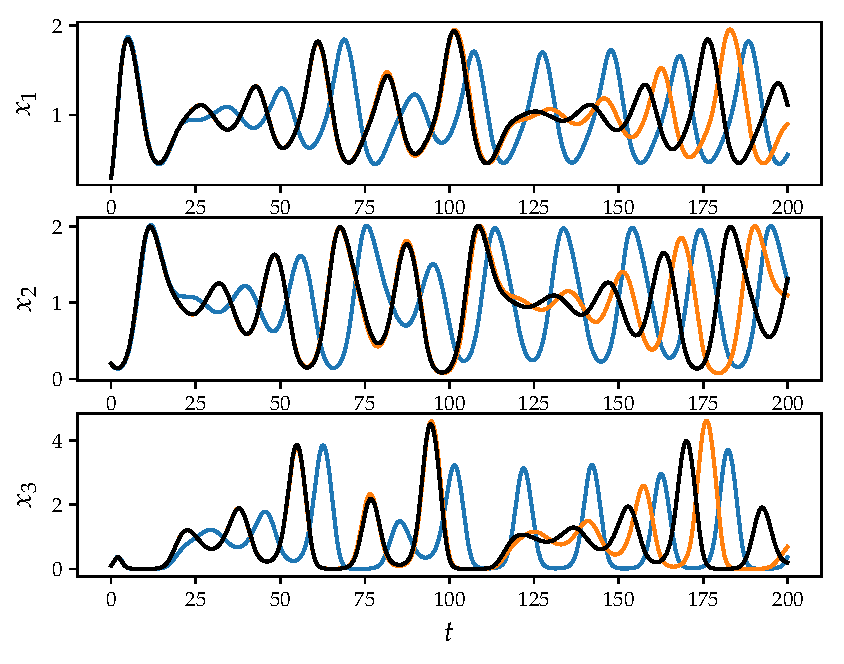
\includegraphics[width=0.35\textwidth]{figs/3SpeciesApprox150_1.pdf}
			&
			\hspace{-5mm}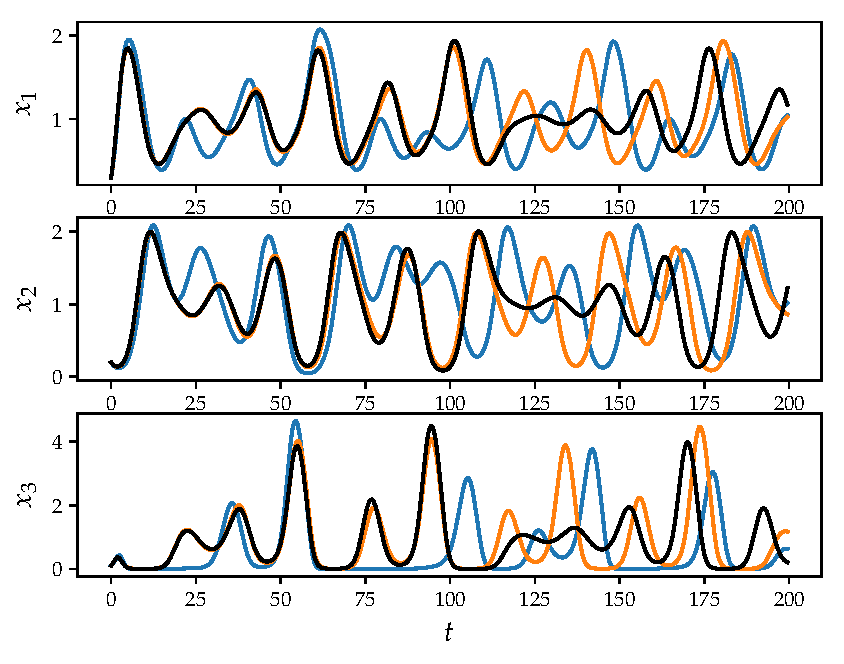
\includegraphics[width=0.35\textwidth]{figs/3SpeciesApprox150_5.pdf}
			&
			\hspace{-5mm}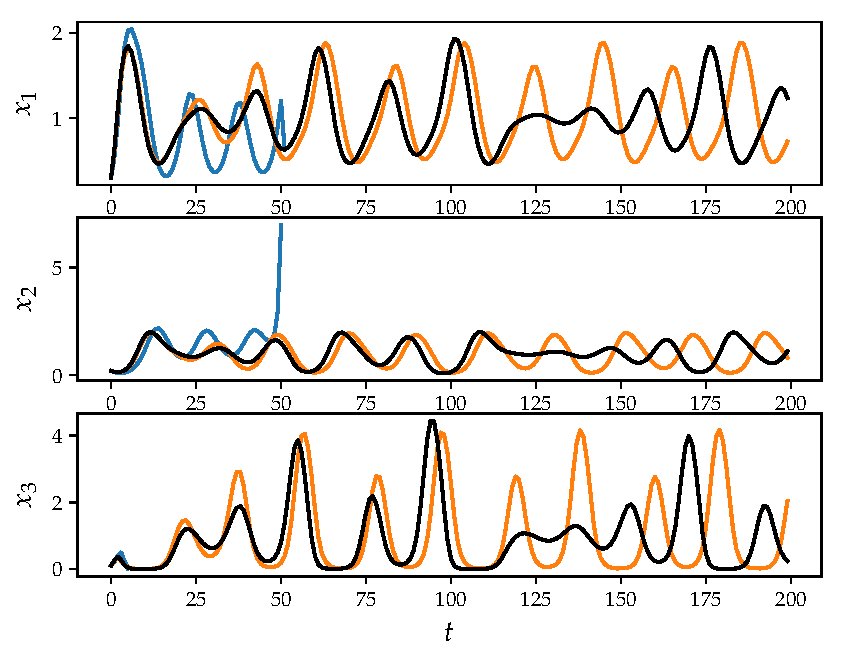
\includegraphics[width=0.35\textwidth]{figs/3SpeciesApprox150_10.pdf}\vspace{-3mm}
			\\
			{\scriptsize \hspace{4mm}(g) $\alpha = 1.50, h=0.1$}&
			{\scriptsize \hspace{4mm}(h) $\alpha = 1.50, h=0.5$}&
			{\scriptsize \hspace{4mm}(i) $\alpha = 1.50, h=1.0$}
		\end{tabular}
		\caption{3-Species Lotka-Volterra system time series for each species $x_i$, estimated using Heun's and Eulers's method, and varying parameters of $\alpha$ and timesteps $h$.}
		\label{9_Lotka-Volterra_plots}
	\end{figure}


	\begin{wrapfigure}{r}{0.65\textwidth}
		\centering
		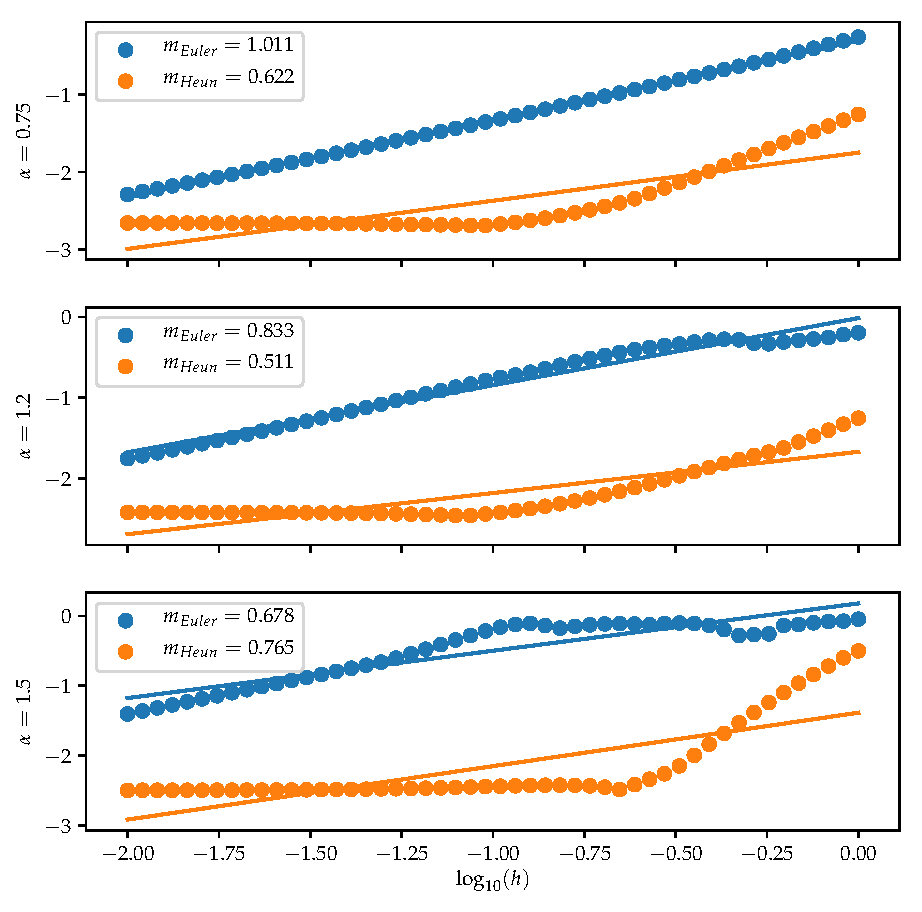
\includegraphics[width=0.7\textwidth]{figs/err_fn.pdf}\vspace{-2mm}
		\caption{Log-log plot of the maximum absolute error in species 1 predictions}
		\label{error_fns}
	\end{wrapfigure}

\prob{3}{To study the error of our integrators we took the difference of the builtin \texttt{solve\_ivp} and the outputs of each of our integrators, \texttt{Euler} and \texttt{Heun}, plotting the maximum absolute differences side by side in Figure \ref{error_fns}. We find, as expected, that the Euler integrator has consistently higher maximum error per timestep spacing, $h$ and also has a higher slope in log-log space. Since the slope of the fit line represents the exponent of the error, although our errors do not match to the theoretical values we believe that this is due to the fact that we are comparing the integrators to builtin function that itself has an error $\sim h^4$. }

\prob{4}{To show the global precision of Heun's method we will start with the limit of the Taylor Series expansion of our function as the function itself, $x(t_{n+1}) = x(t_n) + h f\big(x(t_n)\big) + \frac{h^2}{2}f'\big(x(t_n)\big)$} and then subtract the function estimate from Heun's method at some time step $n+1$ to first get the local precision.
	\begin{align*}
		e_{n+1} &= x(t_{n+1}) - x_H(t_{n+1})
		\\
		&=
		\cancel{x(t_n)} + h f\big(x(t_n)\big) + \frac{h^2}{2}f'\big(x(t_n)\big)
		-
		\bigg(
		\cancel{x(t_n)} + \frac{h}{2}
			\Big[
			f\big(t_n,x(t_n)\big) + f\big(t_{n+1},x_E(t_n)\big)
			\Big]
		\bigg)
		\\
		&\simeq
		h f\big(x(t_n)\big) + \frac{h^2}{2}f'\big(x(t_n)\big)
		-
		\frac{h}{2}
			\Big[
			f\big(x(t_n)\big) + f\big(x(t_n)\big) + h f'\big(x(t_n)\big) + \frac{h^2}{2!}f''\big(x(t_n)\big) + ...
			\Big]
		\\
		&=
		\cancel{h f\big(x(t_n)\big)}
		+
		\cancel{\frac{h^2}{2}f'\big(x(t_n)\big)}
		-
		\Big[
			\cancel{h f\big(x(t_n)\big)}
			+
			\cancel{\frac{h^2}{2} f'\big(x(t_n)\big)}
			+
			\frac{h^3}{4}f''\big(x(t_n)\big)
			+ ...
		\Big]
		\\
		e_{n+1}
		&=
		\boxed{
		-
		\frac{h^3}{4}f''\big(x(t_n)\big)
		+
		\frac{h^4}{2\times3!}f'''\big(x(t_n)\big)...
		}
	\end{align*}
	Since $h \in (0,1)$, $h^3$ is the leading term for our local error and so our local precision scales with $h^3$. Our global precision thus scales as $\boxed{\frac{e_n}{h} = h^2}$.

\prob{5}{
The SIS system is not periodic because the full behavior of the system can be modeled using one equation. In addition, the SIS system lives inside a two-dimensional state space. In order for a system to cycle, it needs to visit a state that is approximately the same as one it has previously visited. This would require the trace of the equation to cross itself at some point, violating the definition of a differentiable function. The SIR and SIRS models however are systems embedded in three dimensions. For each system in $N\geq3$ dimensions, approximately similar states of the system sit on a hyperplane near previously visited states. Since the SIR and SIRS epidemic models are able to be periodic, we can expect that for some set of parameters we would obtain a chaotic system.}
\prob{6}{For the $n$-species Lotka-Volterra model, there are $2^{n}+1$ fixed points. The equation for the deriviative of each species $x_{i}$ is given by
\begin{align*}
    \frac{\mathrm{d}x_{i}}{\mathrm{d}t} &= x_{i}\sum_{j=1}^{n}A_{ij}(1-x_{j})
\end{align*}
Since for each partial derivative $\mathrm{d}x_{i}$ of the system, we fix as constants all other $x_{j}$, the derivative for each $x_{i}$ is a sum of linear functions of the form $cx_{i}$ where each $c=(1-x_{j})A_{ij}$ for $i\neq j$, for which there is a single root of $x_{i}=0$. For the remaining term in the sum of the form $(-x_{i}^{2}+x_{i})A_{ii}$, there are two roots given by the quadratic formula, one of which being $x_{i}=0$. Thus for each partial derivative there are 2 unique solutions to the equation for its derivative. Since the system consists of $n$ species, there are $2^{n}$ fixed points. The final fixed point is given by the state in which all $x_{i}$ are equal to 1, meaning their biomasses have all reached maximum capacity. This is shown for $\alpha=0.75$ in the 3-species model.}
\end{document}
